\documentclass[11pt]{article}
% PACKAGE IMPORTS ----------------------------------------------
\usepackage{geometry}
\usepackage{titling}
\usepackage{enumitem}
\usepackage{ragged2e}
\usepackage{listings}
\usepackage{graphicx}
\usepackage{booktabs}
\usepackage{hyperref}
\usepackage{amsmath}

% FONT SELECTION -----------------------------------------------
\usepackage{tgschola}

% DOCUMENT CONFIGURATION ---------------------------------------
\geometry{letterpaper, margin = 1in}

\pretitle{\noindent \thickrule \skipsmall \centering \bfseries \Huge}
\posttitle{\skipsmall}
\preauthor{\centering \Large}
\postauthor{\skipsmall}
\predate{\centering \Large}
\postdate{\skipsmall \thickrule}

\setlist[enumerate,1]{label=\textbf{\Alph*.}, left = 0.5em, labelsep = 1em}

\lstset{inputencoding=utf8,language=C}
\lstdefinestyle{normal}{basicstyle=\ttfamily\small,breaklines=true,breakatwhitespace=true}
\lstdefinestyle{standalone}{frame=single,numbers=left,basicstyle=\ttfamily\footnotesize,breaklines=true,tabsize=2}

\hypersetup{hidelinks}

\author{Malcolm Riley}

% COMMAND DEFINITIONS ------------------------------------------
\newcommand{\skipsmall}{\vskip 0.5em}
\newcommand{\thickrule}{\rule{\textwidth}{2pt}}
\newcommand{\preparetitle}[1]{\title{Writeup: Homework \##1}}
\setlength{\droptitle}{-30pt}

\newcommand{\code}[1]{\texttt{#1}}
\newcommand{\codesingle}[1]{\begin{center}\fbox{\begin{minipage}{0.85\linewidth}\ttfamily#1\end{minipage}}\end{center}}
\newcommand{\codesample}[1]{\begin{center}\fbox{\begin{minipage}{0.85\linewidth}\lstinputlisting[style=standalone]{#1} \vspace{1em} \centering $\downarrow$ \par \vspace{1em} \input{#1} \\ \vspace{0.5em} \end{minipage}}\end{center}}

\newcommand{\tablehead}[1]{\toprule[2pt]#1\\ \toprule[2pt] \endhead}
\newcommand{\tablefoot}{\bottomrule[2pt]}

\newcommand{\quotes}[1]{``#1''}

\newcommand{\makesection}[2]{\newpage\section*{#1.\quad #2}}
\newcommand{\repolink}{https://github.com/malcolmriley/CMPM-163/blob/master/homework/Assets}
\newcommand{\shaderlink}[1]{\href{\repolink/Shaders/#1.shader}{\texttt{#1.shader}}}
\newcommand{\codelink}[1]{\href{\repolink/Scripts/#1.cs}{\texttt{#1.cs}}}

\newcommand{\makesection}[2]{\newpage\section*{#1.\quad #2}}
\newcommand{\repolink}{https://github.com/malcolmriley/CMPM-163/blob/master/homework/Assets}
\newcommand{\shaderlink}[1]{\href{\repolink/Shaders/#1.shader}{\texttt{#1.shader}}}
\newcommand{\codelink}[1]{\href{\repolink/Scripts/#1.cs}{\texttt{#1.cs}}}

\preparetitle{1}

\begin{document}
\maketitle

\section*{Introduction}
All subtasks of this homework assignment have been integrated into a single Unity scene. No third-party Unity packages were used to create this scene. All code and scene assets including models and sounds were created by myself for the purpose of this assignment.

The viewer can use the mouse to interact with certain objects in the scene. If an object is interactable, a stylized mouse icon will appear in the bottom center of the screen. This is typically used to \quotes{peer} at a particular object in order to get a closer look (with two exceptions). In order to \quotes{lean back} from the \quotes{peering} view and return to the main scene view, right click with the mouse.

The terminal object can be interacted with using the keyboard, navigation controls are displayed on each screen of the terminal. The subtask demonstrations of this homework assignment are accessed through the terminal.

\makesection{A}{Three Objects and Three Lights}
\begin{center}
	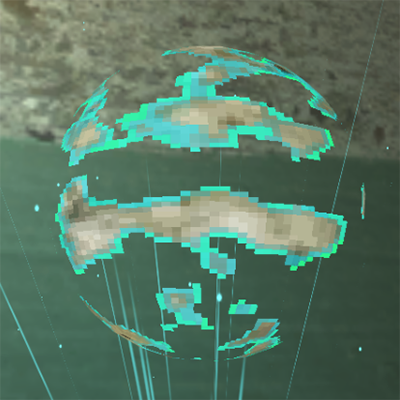
\includegraphics[width=0.3\linewidth]{sphere.png} \quad 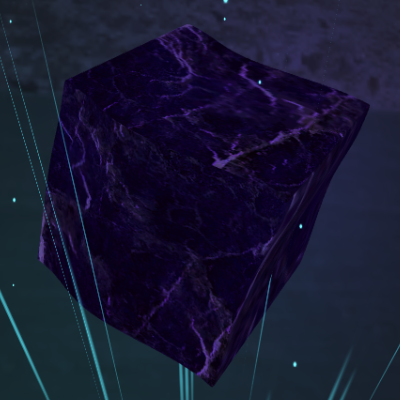
\includegraphics[width=0.3\linewidth]{cube.png} \quad 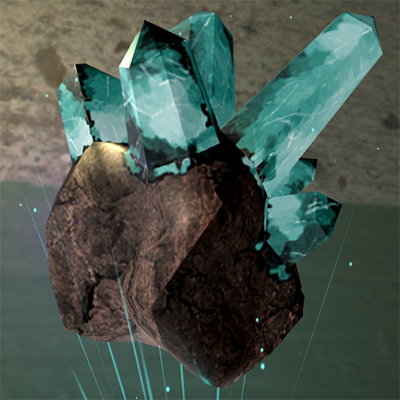
\includegraphics[width=0.3\linewidth]{crystal.png}
\end{center}
The scene contains three lights: One emitted by the hologram projector object, one that revolves around the displayed model, and the lightbulb which may be toggled on or off by left-clicking on the lightswitch object. To access the individual shader demonstrations, activate the terminal and select them from the main menu. The relevant object will be added to the scene as a hovering \quotes{hologram} above the hologram projector object. To inspect the individual objects more closely, left-click on the hologram projector. Click the links in the table below to view the code.
	\begin{center}\begin{tabular}{p{1in}p{2in}p{3in}}
		\toprule
		\textbf{Name} & \textbf{Link to Shader Code} & \textbf{Description} \\ \midrule
		Error Sphere & \shaderlink{Dissolve} & This is an unlit shader that applies a pixelated texture to a sphere, but also a pixelated dissolve effect that changes over time. \\ \midrule
		Cube & \shaderlink{VertexDisplacement} & This is an unlit shader that applies a texture to an object, and deforms the vertices using a sine function. \\ \midrule
		Crystal & \shaderlink{PhongLighting} & This shader applies a texture and the Phong lighting process to an object. It supports up to four point lights. \\
		\bottomrule
	\end{tabular}\end{center}

\makesection{B}{Image Processing Shader}
\begin{center}
	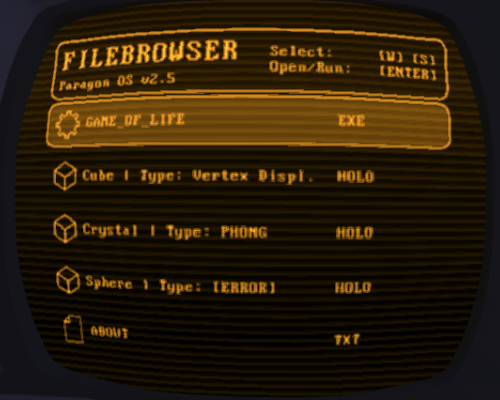
\includegraphics[width=0.5\linewidth]{screeneffect.png}
\end{center}
The kernel-based image processing effect is implemented on the terminal screen object itself. Effectively, it is a standard box blur using a simple $3 \times 3$ convolution matrix. The effect increases over time and may be reset by \quotes{hitting} the terminal by left-clicking on the upper left corner of the terminal object. The intention is to simulate a CRT monitor with malfunctioning deflection coils. The convolution matrix for this effect is defined as:
\[ K = \begin{bmatrix} 1-S & 1-S & 1-S \\ 1-S & S & 1-S \\ 1-S & 1-S & 1-S \end{bmatrix} \] where $S$ is an arbitrary \quotes{sharpness} value. This value is increased over time, thereby biasing the blur effect towards the neighboring pixels. A secondary \code{ScanIntensity} value is dispatched to the shader to control the intensity of the scan lines (themselves being provided by the \code{ScanLines} texture). The shader code can be viewed here: \shaderlink{ScreenEffect}

\makesection{C}{Game of Life \quotes{Ping Pong} Shader}
\begin{center}
	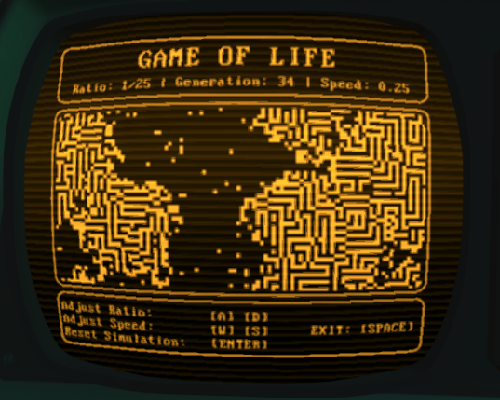
\includegraphics[width=0.5\linewidth]{gameoflife.png}
\end{center}
This shader is implemented as a \quotes{program} within the terminal object and may be accessed by selecting the \quotes{Game of Life} option in the terminal's main menu. The rules of the simulation were discovered as a happy accident during implementation and produce a pleasing, almost mazelike end result. The simulation may be affected within the terminal \quotes{program} by using the controls described on that screen. There are several interoperating parts that are used to accomplish this effect:
\begin{center}\begin{tabular}{p{1in}p{2in}p{3in}}
		\toprule
		\textbf{Name} & \textbf{Link to Code} & \textbf{Description} \\ \midrule
		Game of Life Shader & \shaderlink{GameOfLife} & This is the shader that contains the actual Game of Life Logic. \\ \midrule
		Mask Shader & \shaderlink{SimpleUnlitMasked} & This is the shader that is used to draw the Game of Life result texture onto a field \code{Image} on the terminal screen \code{Canvas}. It simply draws the texture, using the alpha value from a second provided texture. This allows the Game Of Life result texture to be masked. \\ \midrule
		Terminal Screen Code & \codelink{GameOfLifeScreen} & This is the actual \quotes{ping-pong} code that generates and maintains the references to the \code{Texture2D} and \code{RenderTexture} objects and swaps-between them; see the methods \code{GenerateTexture()} \code{OnScreenUpdate()}, respectively.  \\
		\bottomrule
	\end{tabular}\end{center}

\makesection{D}{Visual Effect Discussion}
\begin{center}
	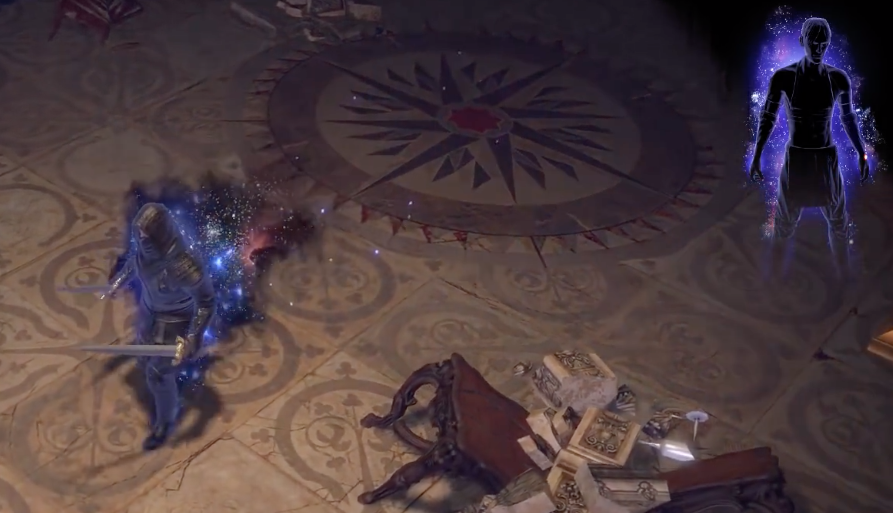
\includegraphics[width=\linewidth]{PoEFX.png}
\end{center}
Depicted above is the \quotes{Celestial Character Effect} from the game \textit{Path of Exile}. A video of the effect may be viewed by clicking the following \href{https://www.youtube.com/watch?v=tiFfWGNF_l8}{\texttt{[YouTube Link]}}. I find this effect to be visually interesting as it contains some pleasing soft particles and strongly invokes the \quotes{celestial} aesthetic. There are several components to the effect:

\begin{itemize}
	\item \textbf{Character Model Highlighting:} This effect appears to be accomplished by the additive application of a bluish color to fragments whose normals are facing away from the camera.
	\item \textbf{Small Soft Particles:} These are simply, as stated, small soft particles of various colors. They appear to be additively blended to the scene during render.
	\item \textbf{Large Soft Particles:} This component is the most sophisticated, and also the most interesting. It appears to have been accomplished by a particle system with a special shader attached. The particle system emits \quotes{smokelike} particles that are then shaded with a static texture of a nebula using the screen-space coordinates of the fragment; this texture is also tiled and offset over time. The alpha of the original particle smoke texture is used.
\end{itemize}

If I were to try and implement this effect using a Unity shader, I would first try to implement the model highlighting as a second pass on top of the standard Unity shader (so that lighting is automatically consistent with the rest of the scene). The highlight color would be exposed as a property of the shader so that it could be altered if later desired. Then, I would implement the large smoky particles as stated above: with a custom shader that uses the alpha of the original particle, and the color value from a tiling, shifting-offset texture whose fragment sample UV parameter is taken from the screen-space of the render target rather than world-space. Finally, I would add the small, soft particles -- they appear to be quite visually similar to Unity's default particles and no custom rendering would be required.

\end{document}